\documentclass[1p]{elsarticle_modified}
%\bibliographystyle{elsarticle-num}

%\usepackage[colorlinks]{hyperref}
%\usepackage{abbrmath_seonhwa} %\Abb, \Ascr, \Acal ,\Abf, \Afrak
\usepackage{amsfonts}
\usepackage{amssymb}
\usepackage{amsmath}
\usepackage{amsthm}
\usepackage{scalefnt}
\usepackage{amsbsy}
\usepackage{kotex}
\usepackage{caption}
\usepackage{subfig}
\usepackage{color}
\usepackage{graphicx}
\usepackage{xcolor} %% white, black, red, green, blue, cyan, magenta, yellow
\usepackage{float}
\usepackage{setspace}
\usepackage{hyperref}

\usepackage{tikz}
\usetikzlibrary{arrows}

\usepackage{multirow}
\usepackage{array} % fixed length table
\usepackage{hhline}

%%%%%%%%%%%%%%%%%%%%%
\makeatletter
\renewcommand*\env@matrix[1][\arraystretch]{%
	\edef\arraystretch{#1}%
	\hskip -\arraycolsep
	\let\@ifnextchar\new@ifnextchar
	\array{*\c@MaxMatrixCols c}}
\makeatother %https://tex.stackexchange.com/questions/14071/how-can-i-increase-the-line-spacing-in-a-matrix
%%%%%%%%%%%%%%%

\usepackage[normalem]{ulem}

\newcommand{\msout}[1]{\ifmmode\text{\sout{\ensuremath{#1}}}\else\sout{#1}\fi}
%SOURCE: \msout is \stkout macro in https://tex.stackexchange.com/questions/20609/strikeout-in-math-mode

\newcommand{\cancel}[1]{
	\ifmmode
	{\color{red}\msout{#1}}
	\else
	{\color{red}\sout{#1}}
	\fi
}

\newcommand{\add}[1]{
	{\color{blue}\uwave{#1}}
}

\newcommand{\replace}[2]{
	\ifmmode
	{\color{red}\msout{#1}}{\color{blue}\uwave{#2}}
	\else
	{\color{red}\sout{#1}}{\color{blue}\uwave{#2}}
	\fi
}

\newcommand{\Sol}{\mathcal{S}} %segment
\newcommand{\D}{D} %diagram
\newcommand{\A}{\mathcal{A}} %arc


%%%%%%%%%%%%%%%%%%%%%%%%%%%%%5 test

\def\sl{\operatorname{\textup{SL}}(2,\Cbb)}
\def\psl{\operatorname{\textup{PSL}}(2,\Cbb)}
\def\quan{\mkern 1mu \triangleright \mkern 1mu}

\theoremstyle{definition}
\newtheorem{thm}{Theorem}[section]
\newtheorem{prop}[thm]{Proposition}
\newtheorem{lem}[thm]{Lemma}
\newtheorem{ques}[thm]{Question}
\newtheorem{cor}[thm]{Corollary}
\newtheorem{defn}[thm]{Definition}
\newtheorem{exam}[thm]{Example}
\newtheorem{rmk}[thm]{Remark}
\newtheorem{alg}[thm]{Algorithm}

\newcommand{\I}{\sqrt{-1}}
\begin{document}

%\begin{frontmatter}
%
%\title{Boundary parabolic representations of knots up to 8 crossings}
%
%%% Group authors per affiliation:
%\author{Yunhi Cho} 
%\address{Department of Mathematics, University of Seoul, Seoul, Korea}
%\ead{yhcho@uos.ac.kr}
%
%
%\author{Seonhwa Kim} %\fnref{s_kim}}
%\address{Center for Geometry and Physics, Institute for Basic Science, Pohang, 37673, Korea}
%\ead{ryeona17@ibs.re.kr}
%
%\author{Hyuk Kim}
%\address{Department of Mathematical Sciences, Seoul National University, Seoul 08826, Korea}
%\ead{hyukkim@snu.ac.kr}
%
%\author{Seokbeom Yoon}
%\address{Department of Mathematical Sciences, Seoul National University, Seoul, 08826,  Korea}
%\ead{sbyoon15@snu.ac.kr}
%
%\begin{abstract}
%We find all boundary parabolic representation of knots up to 8 crossings.
%
%\end{abstract}
%\begin{keyword}
%    \MSC[2010] 57M25 
%\end{keyword}
%
%\end{frontmatter}

%\linenumbers
%\tableofcontents
%
\newcommand\colored[1]{\textcolor{white}{\rule[-0.35ex]{0.8em}{1.4ex}}\kern-0.8em\color{red} #1}%
%\newcommand\colored[1]{\textcolor{white}{ #1}\kern-2.17ex	\textcolor{white}{ #1}\kern-1.81ex	\textcolor{white}{ #1}\kern-2.15ex\color{red}#1	}

{\Large $\underline{10_{70}~(K10a_{22})}$}

\setlength{\tabcolsep}{10pt}
\renewcommand{\arraystretch}{1.6}
\vspace{1cm}\begin{tabular}{m{100pt}>{\centering\arraybackslash}m{274pt}}
\multirow{5}{120pt}{
	\centering
	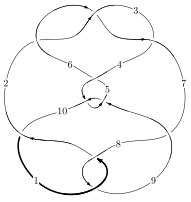
\includegraphics[width=112pt]{../../../GIT/diagram.site/Diagrams/png/154_10_70.png}\\
\ \ \ A knot diagram\footnotemark}&
\allowdisplaybreaks
\textbf{Linearized knot diagam} \\
\cline{2-2}
 &
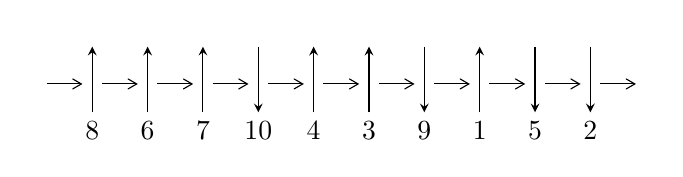
\begin{tikzpicture}[x=20pt, y=17pt]
	% nodes
	\node (C0) at (0, 0) {};
	\node (C1) at (1, 0) {};
	\node (C1U) at (1, +1) {};
	\node (C1D) at (1, -1) {8};

	\node (C2) at (2, 0) {};
	\node (C2U) at (2, +1) {};
	\node (C2D) at (2, -1) {6};

	\node (C3) at (3, 0) {};
	\node (C3U) at (3, +1) {};
	\node (C3D) at (3, -1) {7};

	\node (C4) at (4, 0) {};
	\node (C4U) at (4, +1) {};
	\node (C4D) at (4, -1) {10};

	\node (C5) at (5, 0) {};
	\node (C5U) at (5, +1) {};
	\node (C5D) at (5, -1) {4};

	\node (C6) at (6, 0) {};
	\node (C6U) at (6, +1) {};
	\node (C6D) at (6, -1) {3};

	\node (C7) at (7, 0) {};
	\node (C7U) at (7, +1) {};
	\node (C7D) at (7, -1) {9};

	\node (C8) at (8, 0) {};
	\node (C8U) at (8, +1) {};
	\node (C8D) at (8, -1) {1};

	\node (C9) at (9, 0) {};
	\node (C9U) at (9, +1) {};
	\node (C9D) at (9, -1) {5};

	\node (C10) at (10, 0) {};
	\node (C10U) at (10, +1) {};
	\node (C10D) at (10, -1) {2};
	\node (C11) at (11, 0) {};

	% arrows
	\draw[->,>={angle 60}]
	(C0) edge (C1) (C1) edge (C2) (C2) edge (C3) (C3) edge (C4) (C4) edge (C5) (C5) edge (C6) (C6) edge (C7) (C7) edge (C8) (C8) edge (C9) (C9) edge (C10) (C10) edge (C11) ;	\draw[->,>=stealth]
	(C1D) edge (C1U) (C2D) edge (C2U) (C3D) edge (C3U) (C4U) edge (C4D) (C5D) edge (C5U) (C6D) edge (C6U) (C7U) edge (C7D) (C8D) edge (C8U) (C9U) edge (C9D) (C10U) edge (C10D) ;
	\end{tikzpicture} \\
\hhline{~~} \\& 
\textbf{Solving Sequence} \\ \cline{2-2} 
 &
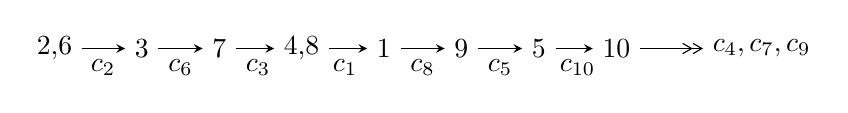
\begin{tikzpicture}[x=28pt, y=7pt]
	% node
	\node (A0) at (-1/8, 0) {2,6};
	\node (A1) at (1, 0) {3};
	\node (A2) at (2, 0) {7};
	\node (A3) at (49/16, 0) {4,8};
	\node (A4) at (33/8, 0) {1};
	\node (A5) at (41/8, 0) {9};
	\node (A6) at (49/8, 0) {5};
	\node (A7) at (57/8, 0) {10};
	\node (C1) at (1/2, -1) {$c_{2}$};
	\node (C2) at (3/2, -1) {$c_{6}$};
	\node (C3) at (5/2, -1) {$c_{3}$};
	\node (C4) at (29/8, -1) {$c_{1}$};
	\node (C5) at (37/8, -1) {$c_{8}$};
	\node (C6) at (45/8, -1) {$c_{5}$};
	\node (C7) at (53/8, -1) {$c_{10}$};
	\node (A8) at (9, 0) {$c_{4},c_{7},c_{9}$};

	% edge
	\draw[->,>=stealth]	
	(A0) edge (A1) (A1) edge (A2) (A2) edge (A3) (A3) edge (A4) (A4) edge (A5) (A5) edge (A6) (A6) edge (A7) ;
	\draw[->>,>={angle 60}]	
	(A7) edge (A8);
\end{tikzpicture} \\ 

\end{tabular} \\

\footnotetext{
The image of knot diagram is generated by the software ``\textbf{Draw programme}" developed by Andrew Bartholomew(\url{http://www.layer8.co.uk/maths/draw/index.htm\#Running-draw}), where we modified some parts for our purpose(\url{https://github.com/CATsTAILs/LinksPainter}).
}\phantom \\ \newline 
\centering \textbf{Ideals for irreducible components\footnotemark of $X_{\text{par}}$} 
 
\begin{align*}
I^u_{1}&=\langle 
- u^{34}+2 u^{33}+\cdots+2 b+1,\;u^{12}-5 u^{10}-2 u^9+9 u^8+8 u^7-4 u^6-10 u^5-6 u^4+2 u^3+5 u^2+a+2 u+1,\\
\phantom{I^u_{1}}&\phantom{= \langle  }u^{35}-3 u^{34}+\cdots+u+1\rangle \\
I^u_{2}&=\langle 
b^2- b+1,\;a+1,\;u+1\rangle \\
\\
\end{align*}
\raggedright * 2 irreducible components of $\dim_{\mathbb{C}}=0$, with total 37 representations.\\
\footnotetext{All coefficients of polynomials are rational numbers. But the coefficients are sometimes approximated in decimal forms when there is not enough margin.}
\newpage
\renewcommand{\arraystretch}{1}
\centering \section*{I. $I^u_{1}= \langle - u^{34}+2 u^{33}+\cdots+2 b+1,\;u^{12}-5 u^{10}+\cdots+a+1,\;u^{35}-3 u^{34}+\cdots+u+1 \rangle$}
\flushleft \textbf{(i) Arc colorings}\\
\begin{tabular}{m{7pt} m{180pt} m{7pt} m{180pt} }
\flushright $a_{2}=$&$\begin{pmatrix}1\\0\end{pmatrix}$ \\
\flushright $a_{6}=$&$\begin{pmatrix}0\\u\end{pmatrix}$ \\
\flushright $a_{3}=$&$\begin{pmatrix}1\\- u^2\end{pmatrix}$ \\
\flushright $a_{7}=$&$\begin{pmatrix}u\\- u^3+u\end{pmatrix}$ \\
\flushright $a_{4}=$&$\begin{pmatrix}- u^2+1\\u^4-2 u^2\end{pmatrix}$ \\
\flushright $a_{8}=$&$\begin{pmatrix}- u^{12}+5 u^{10}+\cdots-2 u-1\\\frac{1}{2} u^{34}- u^{33}+\cdots+u-\frac{1}{2}\end{pmatrix}$ \\
\flushright $a_{1}=$&$\begin{pmatrix}-\frac{1}{2} u^{34}+u^{33}+\cdots- u+\frac{3}{2}\\-\frac{5}{2} u^{34}+4 u^{33}+\cdots+2 u+\frac{3}{2}\end{pmatrix}$ \\
\flushright $a_{9}=$&$\begin{pmatrix}-2 u^{34}+3 u^{33}+\cdots+6 u+1\\\frac{7}{2} u^{34}-6 u^{33}+\cdots-3 u-\frac{5}{2}\end{pmatrix}$ \\
\flushright $a_{5}=$&$\begin{pmatrix}- u^5+2 u^3- u\\u^7-3 u^5+2 u^3+u\end{pmatrix}$ \\
\flushright $a_{10}=$&$\begin{pmatrix}-3 u^{34}+5 u^{33}+\cdots+u+3\\-\frac{5}{2} u^{34}+4 u^{33}+\cdots+2 u+\frac{3}{2}\end{pmatrix}$\\&\end{tabular}
\flushleft \textbf{(ii) Obstruction class $= -1$}\\~\\
\flushleft \textbf{(iii) Cusp Shapes $= -7 u^{34}+7 u^{33}+100 u^{32}-67 u^{31}-665 u^{30}+193 u^{29}+2656 u^{28}+332 u^{27}-6763 u^{26}-4013 u^{25}+10334 u^{24}+13042 u^{23}-5838 u^{22}-22006 u^{21}-10452 u^{20}+17336 u^{19}+25367 u^{18}+3521 u^{17}-19332 u^{16}-18920 u^{15}-1888 u^{14}+11508 u^{13}+11034 u^{12}+2874 u^{11}-3024 u^{10}-4152 u^9-2538 u^8-542 u^7+450 u^6+658 u^5+514 u^4+230 u^3+79 u^2+25 u+8$}\\~\\
\newpage\renewcommand{\arraystretch}{1}
\flushleft \textbf{(iv) u-Polynomials at the component}\newline \\
\begin{tabular}{m{50pt}|m{274pt}}
Crossings & \hspace{64pt}u-Polynomials at each crossing \\
\hline $$\begin{aligned}c_{1},c_{8}\end{aligned}$$&$\begin{aligned}
&u^{35}+2 u^{34}+\cdots-2 u^2+1
\end{aligned}$\\
\hline $$\begin{aligned}c_{2},c_{3},c_{6}\end{aligned}$$&$\begin{aligned}
&u^{35}+3 u^{34}+\cdots+u-1
\end{aligned}$\\
\hline $$\begin{aligned}c_{4},c_{9}\end{aligned}$$&$\begin{aligned}
&u^{35}+u^{34}+\cdots-8 u-4
\end{aligned}$\\
\hline $$\begin{aligned}c_{5}\end{aligned}$$&$\begin{aligned}
&u^{35}-15 u^{34}+\cdots-72 u+16
\end{aligned}$\\
\hline $$\begin{aligned}c_{7},c_{10}\end{aligned}$$&$\begin{aligned}
&u^{35}+12 u^{34}+\cdots+4 u-1
\end{aligned}$\\
\hline
\end{tabular}\\~\\
\newpage\renewcommand{\arraystretch}{1}
\flushleft \textbf{(v) Riley Polynomials at the component}\newline \\
\begin{tabular}{m{50pt}|m{274pt}}
Crossings & \hspace{64pt}Riley Polynomials at each crossing \\
\hline $$\begin{aligned}c_{1},c_{8}\end{aligned}$$&$\begin{aligned}
&y^{35}+12 y^{34}+\cdots+4 y-1
\end{aligned}$\\
\hline $$\begin{aligned}c_{2},c_{3},c_{6}\end{aligned}$$&$\begin{aligned}
&y^{35}-31 y^{34}+\cdots-17 y-1
\end{aligned}$\\
\hline $$\begin{aligned}c_{4},c_{9}\end{aligned}$$&$\begin{aligned}
&y^{35}+15 y^{34}+\cdots-72 y-16
\end{aligned}$\\
\hline $$\begin{aligned}c_{5}\end{aligned}$$&$\begin{aligned}
&y^{35}+7 y^{34}+\cdots-2016 y-256
\end{aligned}$\\
\hline $$\begin{aligned}c_{7},c_{10}\end{aligned}$$&$\begin{aligned}
&y^{35}+24 y^{34}+\cdots+40 y-1
\end{aligned}$\\
\hline
\end{tabular}\\~\\
\newpage\flushleft \textbf{(vi) Complex Volumes and Cusp Shapes}
$$\begin{array}{c|c|c}  
\text{Solutions to }I^u_{1}& \I (\text{vol} + \sqrt{-1}CS) & \text{Cusp shape}\\
 \hline 
\begin{aligned}
u &= -0.827242 + 0.510777 I \\
a &= -1.257960 - 0.317928 I \\
b &= \phantom{-}0.711723 - 0.774742 I\end{aligned}
 & \phantom{-}3.61521 - 1.86508 I & \phantom{-}8.01949 + 2.70414 I \\ \hline\begin{aligned}
u &= -0.827242 - 0.510777 I \\
a &= -1.257960 + 0.317928 I \\
b &= \phantom{-}0.711723 + 0.774742 I\end{aligned}
 & \phantom{-}3.61521 + 1.86508 I & \phantom{-}8.01949 - 2.70414 I \\ \hline\begin{aligned}
u &= -0.943343 + 0.501099 I \\
a &= -0.582372 - 0.149507 I \\
b &= \phantom{-}0.684104 + 0.942114 I\end{aligned}
 & \phantom{-}3.09693 + 3.49535 I & \phantom{-}6.37889 - 3.75014 I \\ \hline\begin{aligned}
u &= -0.943343 - 0.501099 I \\
a &= -0.582372 + 0.149507 I \\
b &= \phantom{-}0.684104 - 0.942114 I\end{aligned}
 & \phantom{-}3.09693 - 3.49535 I & \phantom{-}6.37889 + 3.75014 I \\ \hline\begin{aligned}
u &= -0.253334 + 0.839514 I \\
a &= -1.18782 - 1.13183 I \\
b &= \phantom{-}0.696750 - 1.005540 I\end{aligned}
 & \phantom{-}0.97304 - 8.24742 I & \phantom{-}2.56945 + 7.59916 I \\ \hline\begin{aligned}
u &= -0.253334 - 0.839514 I \\
a &= -1.18782 + 1.13183 I \\
b &= \phantom{-}0.696750 + 1.005540 I\end{aligned}
 & \phantom{-}0.97304 + 8.24742 I & \phantom{-}2.56945 - 7.59916 I \\ \hline\begin{aligned}
u &= -1.15725\phantom{ +0.000000I} \\
a &= -1.05692\phantom{ +0.000000I} \\
b &= \phantom{-}0.346138\phantom{ +0.000000I}\end{aligned}
 & \phantom{-}2.21114\phantom{ +0.000000I} & \phantom{-}4.02480\phantom{ +0.000000I} \\ \hline\begin{aligned}
u &= -0.295449 + 0.784598 I \\
a &= -0.058917 - 0.230488 I \\
b &= \phantom{-}0.766564 + 0.673327 I\end{aligned}
 & \phantom{-}1.97084 - 2.68874 I & \phantom{-}4.58889 + 2.89622 I \\ \hline\begin{aligned}
u &= -0.295449 - 0.784598 I \\
a &= -0.058917 + 0.230488 I \\
b &= \phantom{-}0.766564 - 0.673327 I\end{aligned}
 & \phantom{-}1.97084 + 2.68874 I & \phantom{-}4.58889 - 2.89622 I \\ \hline\begin{aligned}
u &= -1.164960 + 0.288871 I \\
a &= -1.174190 - 0.528323 I \\
b &= \phantom{-}0.051770 - 0.955164 I\end{aligned}
 & -0.612022 - 1.167710 I & -0.594633 + 0.482422 I\\
 \hline 
 \end{array}$$\newpage$$\begin{array}{c|c|c}  
\text{Solutions to }I^u_{1}& \I (\text{vol} + \sqrt{-1}CS) & \text{Cusp shape}\\
 \hline 
\begin{aligned}
u &= -1.164960 - 0.288871 I \\
a &= -1.174190 + 0.528323 I \\
b &= \phantom{-}0.051770 + 0.955164 I\end{aligned}
 & -0.612022 + 1.167710 I & -0.594633 - 0.482422 I \\ \hline\begin{aligned}
u &= -0.098834 + 0.725130 I \\
a &= -0.03188 + 1.73645 I \\
b &= -0.071862 + 1.038610 I\end{aligned}
 & -3.83291 - 2.53588 I & -3.84686 + 3.83326 I \\ \hline\begin{aligned}
u &= -0.098834 - 0.725130 I \\
a &= -0.03188 - 1.73645 I \\
b &= -0.071862 - 1.038610 I\end{aligned}
 & -3.83291 + 2.53588 I & -3.84686 - 3.83326 I \\ \hline\begin{aligned}
u &= \phantom{-}1.275860 + 0.152636 I \\
a &= \phantom{-}0.756171 + 0.131779 I \\
b &= -0.493777 + 1.054750 I\end{aligned}
 & \phantom{-}2.76473 - 0.81126 I & \phantom{-}6.02594 + 0. I\phantom{ +0.000000I} \\ \hline\begin{aligned}
u &= \phantom{-}1.275860 - 0.152636 I \\
a &= \phantom{-}0.756171 - 0.131779 I \\
b &= -0.493777 - 1.054750 I\end{aligned}
 & \phantom{-}2.76473 + 0.81126 I & \phantom{-}6.02594 + 0. I\phantom{ +0.000000I} \\ \hline\begin{aligned}
u &= -1.343360 + 0.175547 I \\
a &= \phantom{-}1.08136 + 1.66784 I \\
b &= -0.750068 - 0.725396 I\end{aligned}
 & \phantom{-}4.76978 - 0.62379 I & \phantom{-}6.88558 + 0. I\phantom{ +0.000000I} \\ \hline\begin{aligned}
u &= -1.343360 - 0.175547 I \\
a &= \phantom{-}1.08136 - 1.66784 I \\
b &= -0.750068 + 0.725396 I\end{aligned}
 & \phantom{-}4.76978 + 0.62379 I & \phantom{-}6.88558 + 0. I\phantom{ +0.000000I} \\ \hline\begin{aligned}
u &= \phantom{-}1.328700 + 0.290772 I \\
a &= \phantom{-}0.892510 - 0.521672 I \\
b &= -0.144398 - 1.112500 I\end{aligned}
 & \phantom{-}0.65547 + 6.20108 I & \phantom{-}1.95124 - 5.89177 I \\ \hline\begin{aligned}
u &= \phantom{-}1.328700 - 0.290772 I \\
a &= \phantom{-}0.892510 + 0.521672 I \\
b &= -0.144398 + 1.112500 I\end{aligned}
 & \phantom{-}0.65547 - 6.20108 I & \phantom{-}1.95124 + 5.89177 I \\ \hline\begin{aligned}
u &= -1.349650 + 0.231790 I \\
a &= \phantom{-}2.67880 - 0.00517 I \\
b &= -0.701280 + 0.976265 I\end{aligned}
 & \phantom{-}4.00753 - 6.15318 I & \phantom{-}5.27676 + 5.00692 I\\
 \hline 
 \end{array}$$\newpage$$\begin{array}{c|c|c}  
\text{Solutions to }I^u_{1}& \I (\text{vol} + \sqrt{-1}CS) & \text{Cusp shape}\\
 \hline 
\begin{aligned}
u &= -1.349650 - 0.231790 I \\
a &= \phantom{-}2.67880 + 0.00517 I \\
b &= -0.701280 - 0.976265 I\end{aligned}
 & \phantom{-}4.00753 + 6.15318 I & \phantom{-}5.27676 - 5.00692 I \\ \hline\begin{aligned}
u &= \phantom{-}1.360060 + 0.198169 I \\
a &= \phantom{-}0.993954 - 0.073655 I \\
b &= -0.734023 - 0.241674 I\end{aligned}
 & \phantom{-}5.16768 + 3.59908 I & \phantom{-}8.99233 - 3.96847 I \\ \hline\begin{aligned}
u &= \phantom{-}1.360060 - 0.198169 I \\
a &= \phantom{-}0.993954 + 0.073655 I \\
b &= -0.734023 + 0.241674 I\end{aligned}
 & \phantom{-}5.16768 - 3.59908 I & \phantom{-}8.99233 + 3.96847 I \\ \hline\begin{aligned}
u &= \phantom{-}0.130391 + 0.566931 I \\
a &= \phantom{-}1.74005 - 1.54748 I \\
b &= -0.611964 - 0.968100 I\end{aligned}
 & -0.69789 + 3.19845 I & -1.06265 - 3.08489 I \\ \hline\begin{aligned}
u &= \phantom{-}0.130391 - 0.566931 I \\
a &= \phantom{-}1.74005 + 1.54748 I \\
b &= -0.611964 + 0.968100 I\end{aligned}
 & -0.69789 - 3.19845 I & -1.06265 + 3.08489 I \\ \hline\begin{aligned}
u &= \phantom{-}1.42263 + 0.31147 I \\
a &= -0.746326 + 1.154990 I \\
b &= \phantom{-}0.845304 - 0.658411 I\end{aligned}
 & \phantom{-}7.44255 + 6.65019 I & \phantom{-0.000000 } 0 \\ \hline\begin{aligned}
u &= \phantom{-}1.42263 - 0.31147 I \\
a &= -0.746326 - 1.154990 I \\
b &= \phantom{-}0.845304 + 0.658411 I\end{aligned}
 & \phantom{-}7.44255 - 6.65019 I & \phantom{-0.000000 } 0 \\ \hline\begin{aligned}
u &= \phantom{-}1.41674 + 0.34279 I \\
a &= -2.20298 + 0.34664 I \\
b &= \phantom{-}0.724315 + 1.038040 I\end{aligned}
 & \phantom{-}6.28512 + 12.51090 I & \phantom{-0.000000 } 0. - 8.16035 I \\ \hline\begin{aligned}
u &= \phantom{-}1.41674 - 0.34279 I \\
a &= -2.20298 - 0.34664 I \\
b &= \phantom{-}0.724315 - 1.038040 I\end{aligned}
 & \phantom{-}6.28512 - 12.51090 I & \phantom{-0.000000 -}0. + 8.16035 I \\ \hline\begin{aligned}
u &= \phantom{-}1.49697 + 0.02263 I \\
a &= -1.77693 - 0.78513 I \\
b &= \phantom{-}0.807430 + 0.880445 I\end{aligned}
 & \phantom{-}11.46670 + 3.01120 I & \phantom{-0.000000 } 0\\
 \hline 
 \end{array}$$\newpage$$\begin{array}{c|c|c}  
\text{Solutions to }I^u_{1}& \I (\text{vol} + \sqrt{-1}CS) & \text{Cusp shape}\\
 \hline 
\begin{aligned}
u &= \phantom{-}1.49697 - 0.02263 I \\
a &= -1.77693 + 0.78513 I \\
b &= \phantom{-}0.807430 - 0.880445 I\end{aligned}
 & \phantom{-}11.46670 - 3.01120 I & \phantom{-0.000000 } 0 \\ \hline\begin{aligned}
u &= -0.223261 + 0.425121 I \\
a &= -0.321375 + 0.194137 I \\
b &= -0.417087 + 0.308331 I\end{aligned}
 & \phantom{-}0.236326 - 1.154630 I & \phantom{-}3.51275 + 5.51426 I \\ \hline\begin{aligned}
u &= -0.223261 - 0.425121 I \\
a &= -0.321375 - 0.194137 I \\
b &= -0.417087 - 0.308331 I\end{aligned}
 & \phantom{-}0.236326 + 1.154630 I & \phantom{-}3.51275 - 5.51426 I \\ \hline\begin{aligned}
u &= \phantom{-}0.146719 + 0.318162 I \\
a &= -0.77364 - 1.20062 I \\
b &= -0.536572 + 0.742317 I\end{aligned}
 & \phantom{-}0.11091 - 1.46996 I & -0.94917 + 3.34118 I \\ \hline\begin{aligned}
u &= \phantom{-}0.146719 - 0.318162 I \\
a &= -0.77364 + 1.20062 I \\
b &= -0.536572 - 0.742317 I\end{aligned}
 & \phantom{-}0.11091 + 1.46996 I & -0.94917 - 3.34118 I\\
 \hline 
 \end{array}$$\newpage\newpage\renewcommand{\arraystretch}{1}
\centering \section*{II. $I^u_{2}= \langle b^2- b+1,\;a+1,\;u+1 \rangle$}
\flushleft \textbf{(i) Arc colorings}\\
\begin{tabular}{m{7pt} m{180pt} m{7pt} m{180pt} }
\flushright $a_{2}=$&$\begin{pmatrix}1\\0\end{pmatrix}$ \\
\flushright $a_{6}=$&$\begin{pmatrix}0\\-1\end{pmatrix}$ \\
\flushright $a_{3}=$&$\begin{pmatrix}1\\-1\end{pmatrix}$ \\
\flushright $a_{7}=$&$\begin{pmatrix}-1\\0\end{pmatrix}$ \\
\flushright $a_{4}=$&$\begin{pmatrix}0\\-1\end{pmatrix}$ \\
\flushright $a_{8}=$&$\begin{pmatrix}-1\\b\end{pmatrix}$ \\
\flushright $a_{1}=$&$\begin{pmatrix}- b+1\\b-1\end{pmatrix}$ \\
\flushright $a_{9}=$&$\begin{pmatrix}0\\b-1\end{pmatrix}$ \\
\flushright $a_{5}=$&$\begin{pmatrix}0\\-1\end{pmatrix}$ \\
\flushright $a_{10}=$&$\begin{pmatrix}0\\b-1\end{pmatrix}$\\&\end{tabular}
\flushleft \textbf{(ii) Obstruction class $= 1$}\\~\\
\flushleft \textbf{(iii) Cusp Shapes $= -4 b+5$}\\~\\
\newpage\renewcommand{\arraystretch}{1}
\flushleft \textbf{(iv) u-Polynomials at the component}\newline \\
\begin{tabular}{m{50pt}|m{274pt}}
Crossings & \hspace{64pt}u-Polynomials at each crossing \\
\hline $$\begin{aligned}c_{1},c_{7},c_{10}\end{aligned}$$&$\begin{aligned}
&u^2- u+1
\end{aligned}$\\
\hline $$\begin{aligned}c_{2},c_{3}\end{aligned}$$&$\begin{aligned}
&(u+1)^2
\end{aligned}$\\
\hline $$\begin{aligned}c_{4},c_{5},c_{9}\end{aligned}$$&$\begin{aligned}
&u^2
\end{aligned}$\\
\hline $$\begin{aligned}c_{6}\end{aligned}$$&$\begin{aligned}
&(u-1)^2
\end{aligned}$\\
\hline $$\begin{aligned}c_{8}\end{aligned}$$&$\begin{aligned}
&u^2+u+1
\end{aligned}$\\
\hline
\end{tabular}\\~\\
\newpage\renewcommand{\arraystretch}{1}
\flushleft \textbf{(v) Riley Polynomials at the component}\newline \\
\begin{tabular}{m{50pt}|m{274pt}}
Crossings & \hspace{64pt}Riley Polynomials at each crossing \\
\hline $$\begin{aligned}c_{1},c_{7},c_{8}\\c_{10}\end{aligned}$$&$\begin{aligned}
&y^2+y+1
\end{aligned}$\\
\hline $$\begin{aligned}c_{2},c_{3},c_{6}\end{aligned}$$&$\begin{aligned}
&(y-1)^2
\end{aligned}$\\
\hline $$\begin{aligned}c_{4},c_{5},c_{9}\end{aligned}$$&$\begin{aligned}
&y^2
\end{aligned}$\\
\hline
\end{tabular}\\~\\
\newpage\flushleft \textbf{(vi) Complex Volumes and Cusp Shapes}
$$\begin{array}{c|c|c}  
\text{Solutions to }I^u_{2}& \I (\text{vol} + \sqrt{-1}CS) & \text{Cusp shape}\\
 \hline 
\begin{aligned}
u &= -1.00000\phantom{ +0.000000I} \\
a &= -1.00000\phantom{ +0.000000I} \\
b &= \phantom{-}0.500000 + 0.866025 I\end{aligned}
 & \phantom{-}1.64493 + 2.02988 I & \phantom{-}3.00000 - 3.46410 I \\ \hline\begin{aligned}
u &= -1.00000\phantom{ +0.000000I} \\
a &= -1.00000\phantom{ +0.000000I} \\
b &= \phantom{-}0.500000 - 0.866025 I\end{aligned}
 & \phantom{-}1.64493 - 2.02988 I & \phantom{-}3.00000 + 3.46410 I\\
 \hline 
 \end{array}$$\newpage
\newpage\renewcommand{\arraystretch}{1}
\centering \section*{ III. u-Polynomials}
\begin{tabular}{m{50pt}|m{274pt}}
Crossings & \hspace{64pt}u-Polynomials at each crossing \\
\hline $$\begin{aligned}c_{1}\end{aligned}$$&$\begin{aligned}
&(u^2- u+1)(u^{35}+2 u^{34}+\cdots-2 u^2+1)
\end{aligned}$\\
\hline $$\begin{aligned}c_{2},c_{3}\end{aligned}$$&$\begin{aligned}
&((u+1)^2)(u^{35}+3 u^{34}+\cdots+u-1)
\end{aligned}$\\
\hline $$\begin{aligned}c_{4},c_{9}\end{aligned}$$&$\begin{aligned}
&u^2(u^{35}+u^{34}+\cdots-8 u-4)
\end{aligned}$\\
\hline $$\begin{aligned}c_{5}\end{aligned}$$&$\begin{aligned}
&u^2(u^{35}-15 u^{34}+\cdots-72 u+16)
\end{aligned}$\\
\hline $$\begin{aligned}c_{6}\end{aligned}$$&$\begin{aligned}
&((u-1)^2)(u^{35}+3 u^{34}+\cdots+u-1)
\end{aligned}$\\
\hline $$\begin{aligned}c_{7},c_{10}\end{aligned}$$&$\begin{aligned}
&(u^2- u+1)(u^{35}+12 u^{34}+\cdots+4 u-1)
\end{aligned}$\\
\hline $$\begin{aligned}c_{8}\end{aligned}$$&$\begin{aligned}
&(u^2+u+1)(u^{35}+2 u^{34}+\cdots-2 u^2+1)
\end{aligned}$\\
\hline
\end{tabular}\newpage\renewcommand{\arraystretch}{1}
\centering \section*{ IV. Riley Polynomials}
\begin{tabular}{m{50pt}|m{274pt}}
Crossings & \hspace{64pt}Riley Polynomials at each crossing \\
\hline $$\begin{aligned}c_{1},c_{8}\end{aligned}$$&$\begin{aligned}
&(y^2+y+1)(y^{35}+12 y^{34}+\cdots+4 y-1)
\end{aligned}$\\
\hline $$\begin{aligned}c_{2},c_{3},c_{6}\end{aligned}$$&$\begin{aligned}
&((y-1)^2)(y^{35}-31 y^{34}+\cdots-17 y-1)
\end{aligned}$\\
\hline $$\begin{aligned}c_{4},c_{9}\end{aligned}$$&$\begin{aligned}
&y^2(y^{35}+15 y^{34}+\cdots-72 y-16)
\end{aligned}$\\
\hline $$\begin{aligned}c_{5}\end{aligned}$$&$\begin{aligned}
&y^2(y^{35}+7 y^{34}+\cdots-2016 y-256)
\end{aligned}$\\
\hline $$\begin{aligned}c_{7},c_{10}\end{aligned}$$&$\begin{aligned}
&(y^2+y+1)(y^{35}+24 y^{34}+\cdots+40 y-1)
\end{aligned}$\\
\hline
\end{tabular}
\vskip 2pc
\end{document}